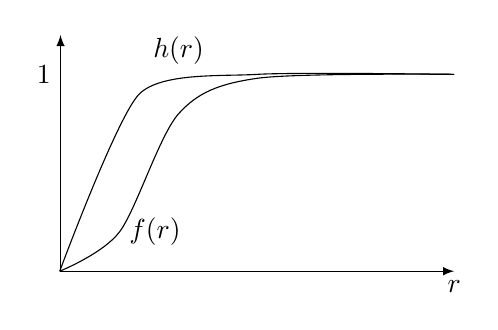
\begin{tikzpicture}

\draw [-latex] (0,-0.01) -- (0,3) ;
\draw [-latex] (-0.01,0) node (v1) {} -- (5,0);

\node (v3) at (2.5,2.5) {};
\node (v2) at (1,2.25) {};
\draw  plot[smooth, tension=0.4] coordinates {(v1) (v2) (v3) (5,2.5) };
\node [right] (v4) at (0.75,0.5) {$f(r)$};
\draw  plot[smooth, tension=.5] coordinates {(v1) (0.75,0.5) (1.5,2) (2.5,2.45) (5,2.5) };

\node at (1.5,2) {};
\node (v5) at (5,2.5) {};
\node [below] at (5,0) {$r$};
\node [above] at (1.5,2.5) {$h(r)$};
\node [left] at (0,2.5) {$1$};
\end{tikzpicture}